% LaTeX template for Models of Computation assessed coursework
% Most of the required packages are standard and should be provided by most TeX installations

% This file is released into the Public Domain

\documentclass[11pt,a4paper]{article}

\usepackage{fullpage}
\usepackage{rotating}
\usepackage{amsmath, amssymb, amsthm}
\usepackage{stmaryrd}
\usepackage{tikz}
\usepackage{verbatim}
\usepackage{url}
\usepackage{multicol}
\usepackage{xr-hyper}

\usetikzlibrary{automata}
\usetikzlibrary{arrows}
\usetikzlibrary{snakes}

\newcommand{\ang}[1]{\langle #1 \rangle}
\newcommand{\ra}{\rightarrow}

% Register Machines
\newcommand{\START}{\mathit{START}}
\newcommand{\HALT}{\mathit{HALT}}

\newcommand{\uinc}[2]{#1^+ \ra L_{#2}}
\newcommand{\udec}[3]{#1^- \ra L_{#2}, L_{#3}}

\newcommand{\iinc}[3]{L_{#1} & : \uinc{#2}{#3} \\}
\newcommand{\idec}[4]{L_{#1} & : \udec{#2}{#3}{#4} \\}
\newcommand{\ihalt}[1]{L_{#1} & : \HALT \\}

\newcommand{\code}[1]{\ulcorner{#1}\urcorner}
\newcommand{\ppair}[1]{\langle\hspace{-0.6ex}\langle #1 \rangle\hspace{-0.6ex}\rangle}
\newcommand{\pair}[1]{\ang{#1}}

\begin{document}
\title{Models of Computation Assessed Coursework II}
\author{A. Student}

\maketitle

This document is a skeleton which provides macros to help typeset your solution to the coursework.

Register machine rules can be typeset like this:
  \[ \begin{array}{r@{\ }l}
    \idec{0}{R_1}{3}{5}
    \idec{1}{R_1}{4}{2}
    \ihalt{2}
    \idec{3}{R_1}{1}{2}
    \iinc{4}{R_0}{0}
    \ihalt{5}
  \end{array} \]

Pairs and encodings:
\begin{gather*}
    \ppair{1,2} \\
    \pair{3,4} \\
    \code{[1,2,3,4]} = \ppair{1,\ppair{2,\ppair{3,\ppair{4,0}}}} \\
    \code{\uinc{R_1}{2}}
\end{gather*}

Graphing a register machine:
    \begin{center}
        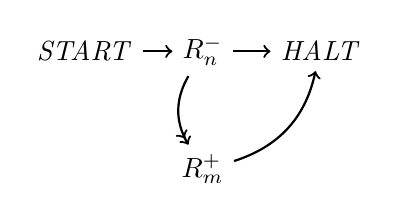
\begin{tikzpicture}[baseline=(current bounding box.center),node distance=1.5cm,thick]
          \node (S) {$\START$};
          \node (L0) [right of=S] {$R_n^-$};
          \node (L1) [right of=L0] {$\HALT$};
          \node (L2) [below of=L0] {$R_m^+$};
          \path[->] (S) edge (L0)
                    (L0) edge (L1) edge[bend right,->>] (L2)
                    (L2) edge[bend right] (L1);
        \end{tikzpicture}
    \end{center}

Other useful notation:
\begin{gather*}
    \mathbb{N} \\
    n_\phi
\end{gather*}


\end{document}
